\section{RK键盘说明书}
\href{http://www.rkgaming.com/zh-CN/article.php?id=115}{说明书链接}, 型号\emphasizebox{RK104Plus}, 谢您选择RK产品,为能使您快速了解并掌握本产品,敬请您务必仔细阅读本操作使用指南,若本操作说明书不够详细或令您不够理解,尽请拔打服务热线400-829-7770,我们的服务人员将会热心解答您的疑问。本产品兼容 Windows2000、XP Vista、Win7、Win8、Win10、MacOS、Android及ios等系统设备。
\begin{figure}[H]
\centering
%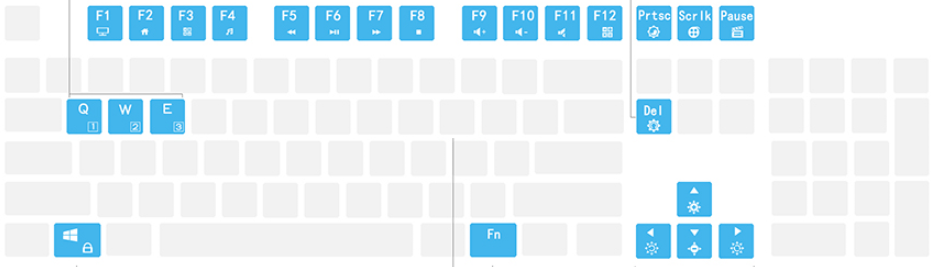
\includegraphics[height=8cm]{keyboard_01.png}
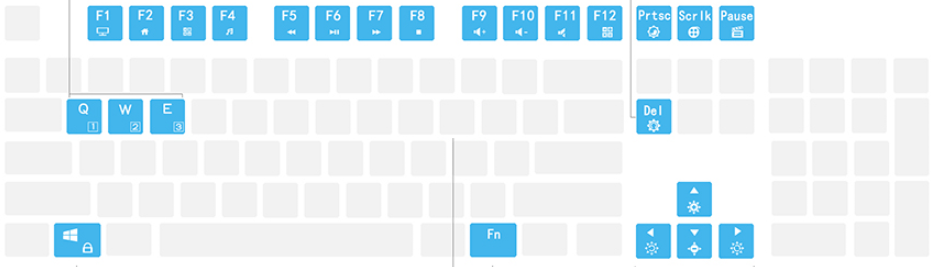
\includegraphics[scale=0.6]{keyboard_01.png}
\caption{键盘模拟图}
\end{figure}

\subsection{多媒体快捷键}
\begin{messagebox}
Fn+F1 计算机, Fn+F5 上一曲, Fn+F9 音量+
Fn+F2 浏览器, Fn+F6 下一曲, Fn+F10 音量-
Fn+F3 邮箱, Fn+F7 播放/暂停, Fn+F11 静音
Fn+F4 播放器, Fn+F8 停止, Fn+F12 计算器
\end{messagebox}

\subsection{三模(蓝牙/2.4G/有线)切换/配对方法}
\begin{itemize}
\item 有线模式:连接USB至设备,自动强制切换为有线模式(无论背部开关处于任何状态)
\item 2.4G模式:如下图,键盘背部两个开关,开关1拨到ON状态,开关2拨到G状态。
2.4G配对方法:开关1拨到ON状态,开关2拨到G状态。FN+P长按对码,P键闪烁插入接收器,P键停止闪烁即对码成功。
(温馨提示:出厂时已配对好接收器,无需自行再次配对2.4G;次方法只是2.4G无法连接的时候使用,首次设置即可,无需每次都设置)
\item 蓝牙配对方法:
\begin{messagebox}
1.开关1拨到ON状态,开关2拨到B状态
2.FN+Q/W/E/R/T.任意一组长按对码,比如Fn+Q,此时Q键持续闪烁闪烁,表示已进入配对状态
3.打开设备蓝牙(电脑/手机/平板)搜索名为:RK-Three mode keyboard的设备
4.完成连接
以此类推:重复以上步骤,Q/W/E/R/T 可存储5组蓝牙设备,在使用切换时短按Fn+Q/W/E/R/T,
即可在不同蓝牙设备之间切换(温馨提示:使用切换前,请先配对好5组蓝牙)
\end{messagebox}
\end{itemize}

\subsection{背光设置}
\begin{itemize}
\item Fn+Prtsc 17种背光效果切换, 可切换17种背光效果,依次为:常亮、呼吸、流光、下落、环形跑马、雨滴、涟漪、繁星、一字跑马、斜上跑马、左右穿插、单点亮、单点灭,波浪、环形绽放、一字绽放、劈开。
\item 自定义背光录制, Fn+Scrlk 支持三组自定义背光切换:此功能可切换三组自定义背光, Fn+Pause 录制自定义背光, 具体操作方法:
\begin{messagebox}
1.先通过Fn+Scrlk选择一组将要自定义的背光
2.按下Fn+pause进入背光录制模式,此时键盘指示灯持续闪烁,表示已开始录制背光
3.按下想要录制背光的按键(按一下亮,再按一下灭),重复此步骤,录制自己想要的背光
4.完成后,再次按下Fn+pause,将保存并退出背光录制模式
以此类推,重复以上步骤可录制三种自定义背光,并且可通过Fn+scrlk随时切换
\end{messagebox}

\item 背光亮度/速度设置, Fn+↑ 背光亮度增加, 共五档调节,调节到最大峰值时,指示灯将连续闪烁三次,表明已到最大亮度, Fn+↓ 背光亮度减小, 共五档调节,支持关闭背光,调节到最小峰值时,指示灯将连续闪烁三次,表明已到最小亮度(背光关闭)。Fn+← 背光速度减小, 共五档调节,调节到最小峰值时,指示灯将连续闪烁三次,表明已到最小速度, Fn+→动态变幻速度增加,共五档调节,调节到最达峰值时,指示灯将连续闪烁三次,表明已到最大速度。
\end{itemize}

\subsection{其他设置}
Fn+Win 锁定/解锁win键, 在键盘使用过程中,为了防止误触windows键,可通过Fn+Win停用/启用windows键功能, Fn+Del 恢复出厂设置, 在键盘使用过程中,可通过Fn+Del恢复出厂设置,此时会默认为出厂状态,之前连接的蓝牙设备、自定义背光等都会被清除。


\subsection{充电说明}
温馨提示:本产品不配备充电器,可连接手机充电器或者电脑USB进行充电
\begin{messagebox}
1.为保障您的正常使用,第一次使用本产品前请您对产品进行充电。当您随身携带本产品时,
请将产品背面开关调至off状态以便省电。
2.电量过低时,Fn键背光会持续闪烁,此时请连接充电器进行充电。
3.充电器充电时注意不可大于5V 1A,也可以直接插在电脑USB上充电
4.充电时空格红灯常亮,充满熄灭,三小时左右充满,不可为了加速充电而使用大于5V1A的
充电器,否则电池寿命会有一定的损坏和影响。
\end{messagebox}

\subsection{节能省电}
关闭键盘:背部开关拨至OFF, 本产品一分钟无操作,键盘背光自动关闭;五分钟无操作,键盘进入待机状态;十分钟无操作,键盘进入深度休眠,唤醒键盘仅需按任意键。
